\RequirePackage[l2tabu,orthodox]{nag}

% two-sided
\documentclass[headsepline,footsepline,footinclude=false,fontsize=11pt,paper=a4,listof=totoc,bibliography=totoc,BCOR=12mm,DIV=12]{scrbook} % two-sided
% \documentclass[headsepline,footsepline,footinclude=false,oneside,fontsize=11pt,paper=a4,listof=totoc,bibliography=totoc]{scrbook} % one-sided

\PassOptionsToPackage{table,svgnames,dvipsnames}{xcolor}

\usepackage[utf8]{inputenc}
\usepackage[T1]{fontenc}
\usepackage[sc]{mathpazo}
\usepackage[ngerman,american]{babel}
\usepackage[autostyle]{csquotes}
\usepackage[%
  backend=biber,
  url=false,
  sorting=ynt,
  style=numeric,
  maxnames=4,
  minnames=3,
  maxbibnames=99,
  giveninits,
  uniquename=init]{biblatex}
\usepackage{graphicx}
\usepackage{scrhack} % necessary for listings package
\usepackage{listings}
\usepackage{lstautogobble}
\usepackage{tikz}
\usepackage{pgfplots}
\usepackage{pgfplotstable}
\usepackage{booktabs}
\usepackage[final]{microtype}
\usepackage{caption}
\usepackage[hidelinks]{hyperref} % hidelinks removes colored boxes around references and links
\usepackage{amsmath}
\usepackage{mathtools}
\usepackage{amsthm,thmtools}
\usepackage[nottoc]{tocbibind}
\usepackage[ruled]{algorithm2e}
\usepackage{enumerate}
\usepackage{tabularx}
% \usepackage{ltablex}
\usepackage{imakeidx}

\DeclareMathOperator*{\argmax}{arg\,max}
\DeclareMathOperator*{\argmin}{arg\,min}

\makeindex[intoc]

\DeclarePairedDelimiter{\norm}{\lVert}{\rVert}

\declaretheorem[name=Theorem]{theorem}
\declaretheorem[name=Lemma,sibling=theorem]{lemma}
\declaretheorem[name=Definition,sibling=theorem]{definition}
\declaretheorem[name=Problem,sibling=theorem]{problem}
\makeatletter
\def\ll@problem{
  \protect\numberline{\theproblem}\thmt@shortoptarg
}
\makeatother

\renewcommand{\thealgocf}{\arabic{theorem}}

\bibliography{sources}

\setkomafont{disposition}{\normalfont\bfseries} % use serif font for headings
\linespread{1.05} % adjust line spread for mathpazo font

% Add table of contents to PDF bookmarks
\BeforeTOCHead[toc]{{\cleardoublepage\pdfbookmark[0]{\contentsname}{toc}}}

% Define TUM corporate design colors
% Taken from http://portal.mytum.de/corporatedesign/index_print/vorlagen/index_farben
\definecolor{TUMBlue}{HTML}{0065BD}
\definecolor{TUMSecondaryBlue}{HTML}{005293}
\definecolor{TUMSecondaryBlue2}{HTML}{003359}
\definecolor{TUMBlack}{HTML}{000000}
\definecolor{TUMWhite}{HTML}{FFFFFF}
\definecolor{TUMDarkGray}{HTML}{333333}
\definecolor{TUMGray}{HTML}{808080}
\definecolor{TUMLightGray}{HTML}{CCCCC6}
\definecolor{TUMAccentGray}{HTML}{DAD7CB}
\definecolor{TUMAccentOrange}{HTML}{E37222}
\definecolor{TUMAccentGreen}{HTML}{A2AD00}
\definecolor{TUMAccentLightBlue}{HTML}{98C6EA}
\definecolor{TUMAccentBlue}{HTML}{64A0C8}

% Settings for pgfplots
\pgfplotsset{compat=newest}
\pgfplotsset{
  % For available color names, see http://www.latextemplates.com/svgnames-colors
  cycle list={TUMBlue\\TUMAccentOrange\\TUMAccentGreen\\TUMSecondaryBlue2\\TUMDarkGray\\},
}

% Settings for lstlistings
\lstset{%
  basicstyle=\ttfamily,
  columns=fullflexible,
  autogobble,
  keywordstyle=\bfseries\color{TUMBlue},
  stringstyle=\color{TUMAccentGreen}
}

% Colors
\def\b{\textcolor{blue}}
\def\r{\textcolor{red}}

% Ternary operator
\newcommand{\ternary}[3]{\textbf{if}\ #1\ \textbf{then}\ #2\ \textbf{else}\ #3}


% thesis information
\newcommand*{\getUniversity}{Technical University of Munich}
\newcommand*{\getFaculty}{Department of Informatics}
\newcommand*{\getTitle}{Implementation of Algorithms for Right-Sizing Data Centers}
\newcommand*{\getTitleGer}{Implementierung von Algorithmen für die Größenanpassung von Rechenzentren}
\newcommand*{\getAuthor}{Jonas Hübotter}
\newcommand*{\getDoctype}{Bachelor's Thesis in Informatics}
\newcommand*{\getSupervisor}{Prof. Dr. Susanne Albers}
\newcommand*{\getAdvisor}{Jens Quedenfeld}
\newcommand*{\getSubmissionDate}{July 31, 2021}
\newcommand*{\getSubmissionLocation}{Munich}

\makenoidxglossaries

% basic notation
\glsxtrnewsymbol[description={\ensuremath{\{1, \dots, n\}}, for \ensuremath{n \in \mathbb{N}}}]{range}{\ensuremath{[n]}}
\glsadd{range}
\glsxtrnewsymbol[description={\ensuremath{\{0\} \cup [n]}, for \ensuremath{n \in \mathbb{N}}}]{0range}{\ensuremath{[n]_0}}
\glsadd{0range}
\glsxtrnewsymbol[description={\ensuremath{\max\{0, x\}}, for \ensuremath{x \in \mathbb{R}}}]{positive}{\ensuremath{(x)^+}}
\glsadd{positive}
\glsxtrnewsymbol[description={smallest entry of the vector \ensuremath{x}}]{vec_min}{\ensuremath{x_{min}}}
\glsadd{vec_min}
\glsxtrnewsymbol[description={largest entry of the vector \ensuremath{x}}]{vec_max}{\ensuremath{x_{max}}}
\glsadd{vec_max}

% symbols


\begin{document}

% Set page numbering to avoid "destination with the same identifier has been already used" warning for cover page.
% (see https://en.wikibooks.org/wiki/LaTeX/Hyperlinks#Problems_with_Links_and_Pages).
\pagenumbering{alph}
\begin{titlepage}
  % HACK for two-sided documents: ignore binding correction for cover page.
  % Adapted from Markus Kohm's KOMA-Script titlepage=firstiscover handling.
  % See http://mirrors.ctan.org/macros/latex/contrib/koma-script/scrkernel-title.dtx,
  % \maketitle macro.
  \oddsidemargin=\evensidemargin\relax
  \textwidth=\dimexpr\paperwidth-2\evensidemargin-2in\relax
  \hsize=\textwidth\relax

  \centering
  \null
  \vspace{18mm}
  \IfFileExists{thesis/logos/tum.pdf}{%
    
\includegraphics[height=20mm]{thesis/logos/tum.pdf}
  }{%
    \vspace*{20mm}
  }

  \vspace{10mm}
  {\huge\MakeUppercase{\getFaculty{}}}\\

  \vspace{5mm}
  {\large\MakeUppercase{\getUniversity{}}}\\

  \vspace{20mm}
  {\Large \getDoctype{}}

  \vspace{15mm}
  {\huge\bfseries \getTitle{}}

  \vspace{15mm}
  {\LARGE \getAuthor{}}

  \IfFileExists{thesis/logos/faculty.pdf}{%
    \vfill{}
    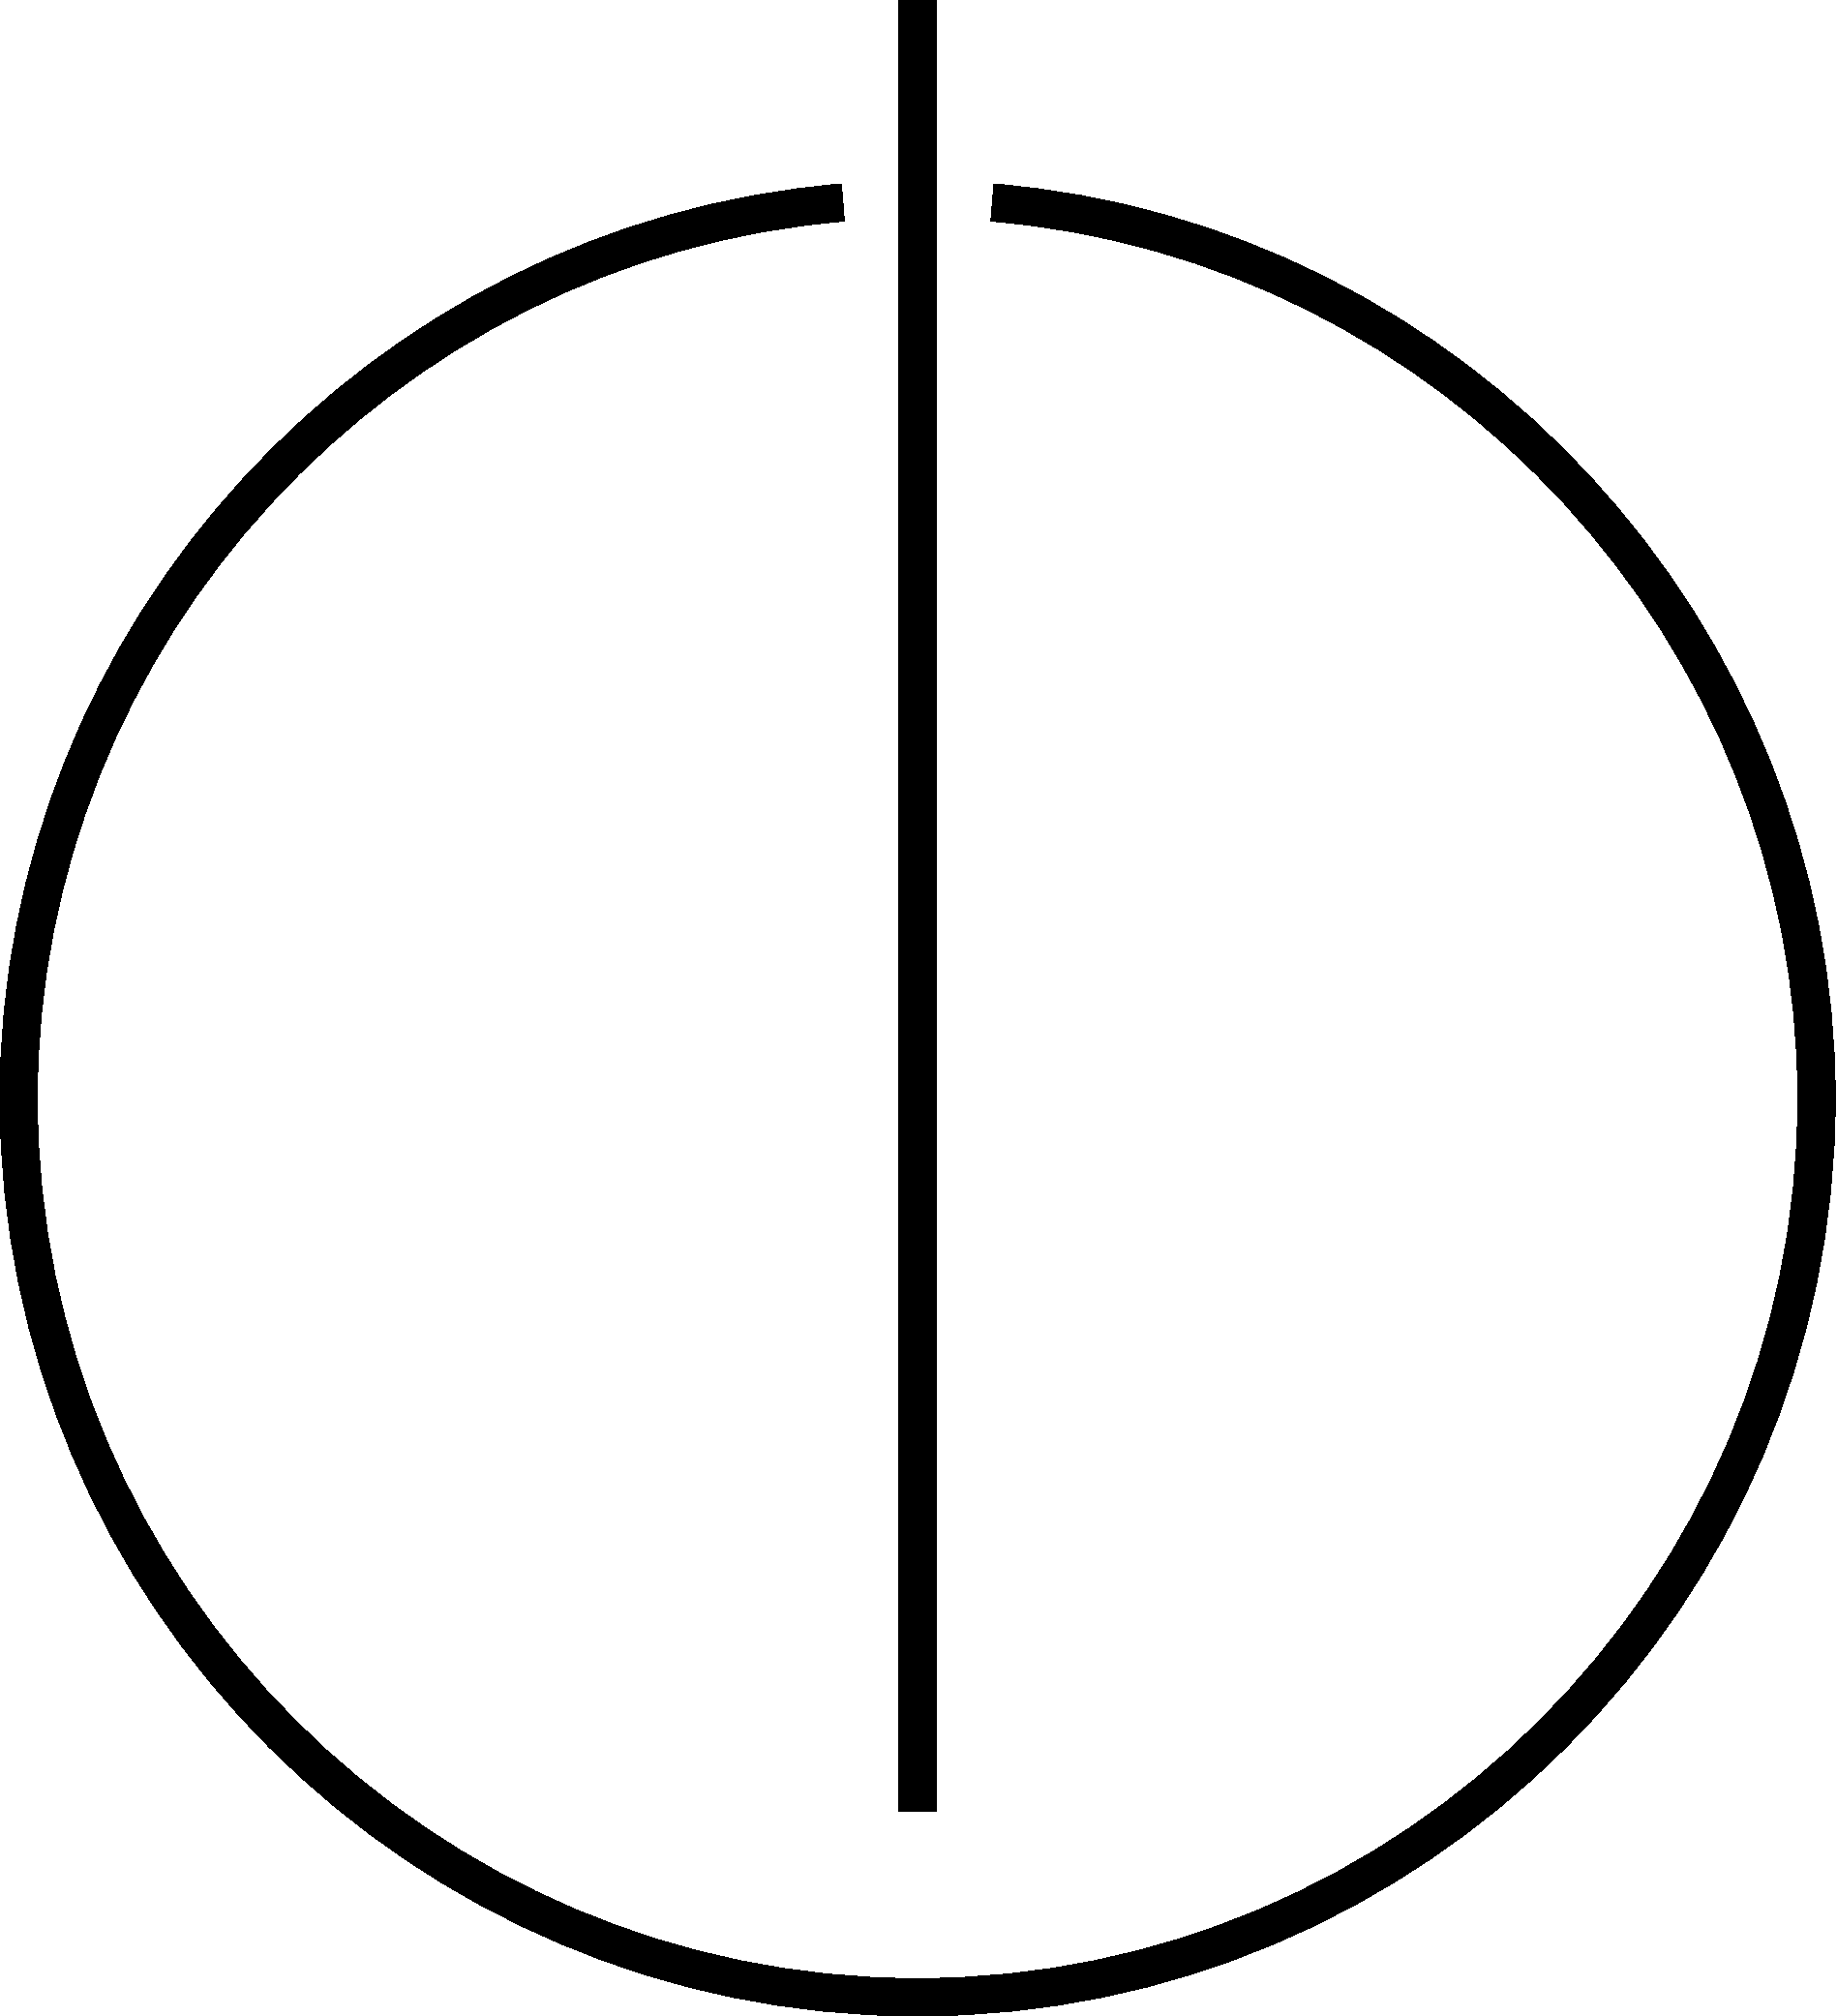
\includegraphics[height=20mm]{thesis/logos/faculty.pdf}
  }{}
\end{titlepage}

\frontmatter{}

\begin{titlepage}
  \centering

  \IfFileExists{thesis/logos/tum.pdf}{%
    
\includegraphics[height=20mm]{thesis/logos/tum.pdf}
  }{%
    \vspace*{20mm}
  }

  \vspace{10mm}
  {\huge\MakeUppercase{\getFaculty{}}}\\

  \vspace{5mm}
  {\large\MakeUppercase{\getUniversity{}}}\\

  \vspace{20mm}
  {\Large \getDoctype{}}

  \vspace{15mm}
  {\huge\bfseries \getTitle{}}

  \vspace{10mm}
  {\huge\bfseries \foreignlanguage{ngerman}{\getTitleGer{}}}

  \vspace{15mm}
  \begin{tabular}{l l}
    Author:          & \getAuthor{} \\
    Supervisor:      & \getSupervisor{} \\
    Advisor:         & \getAdvisor{} \\
    Submission Date: & \getSubmissionDate{} \\
  \end{tabular}

  \vspace{6mm}
  \IfFileExists{thesis/logos/faculty.pdf}{%
    \vfill{}
    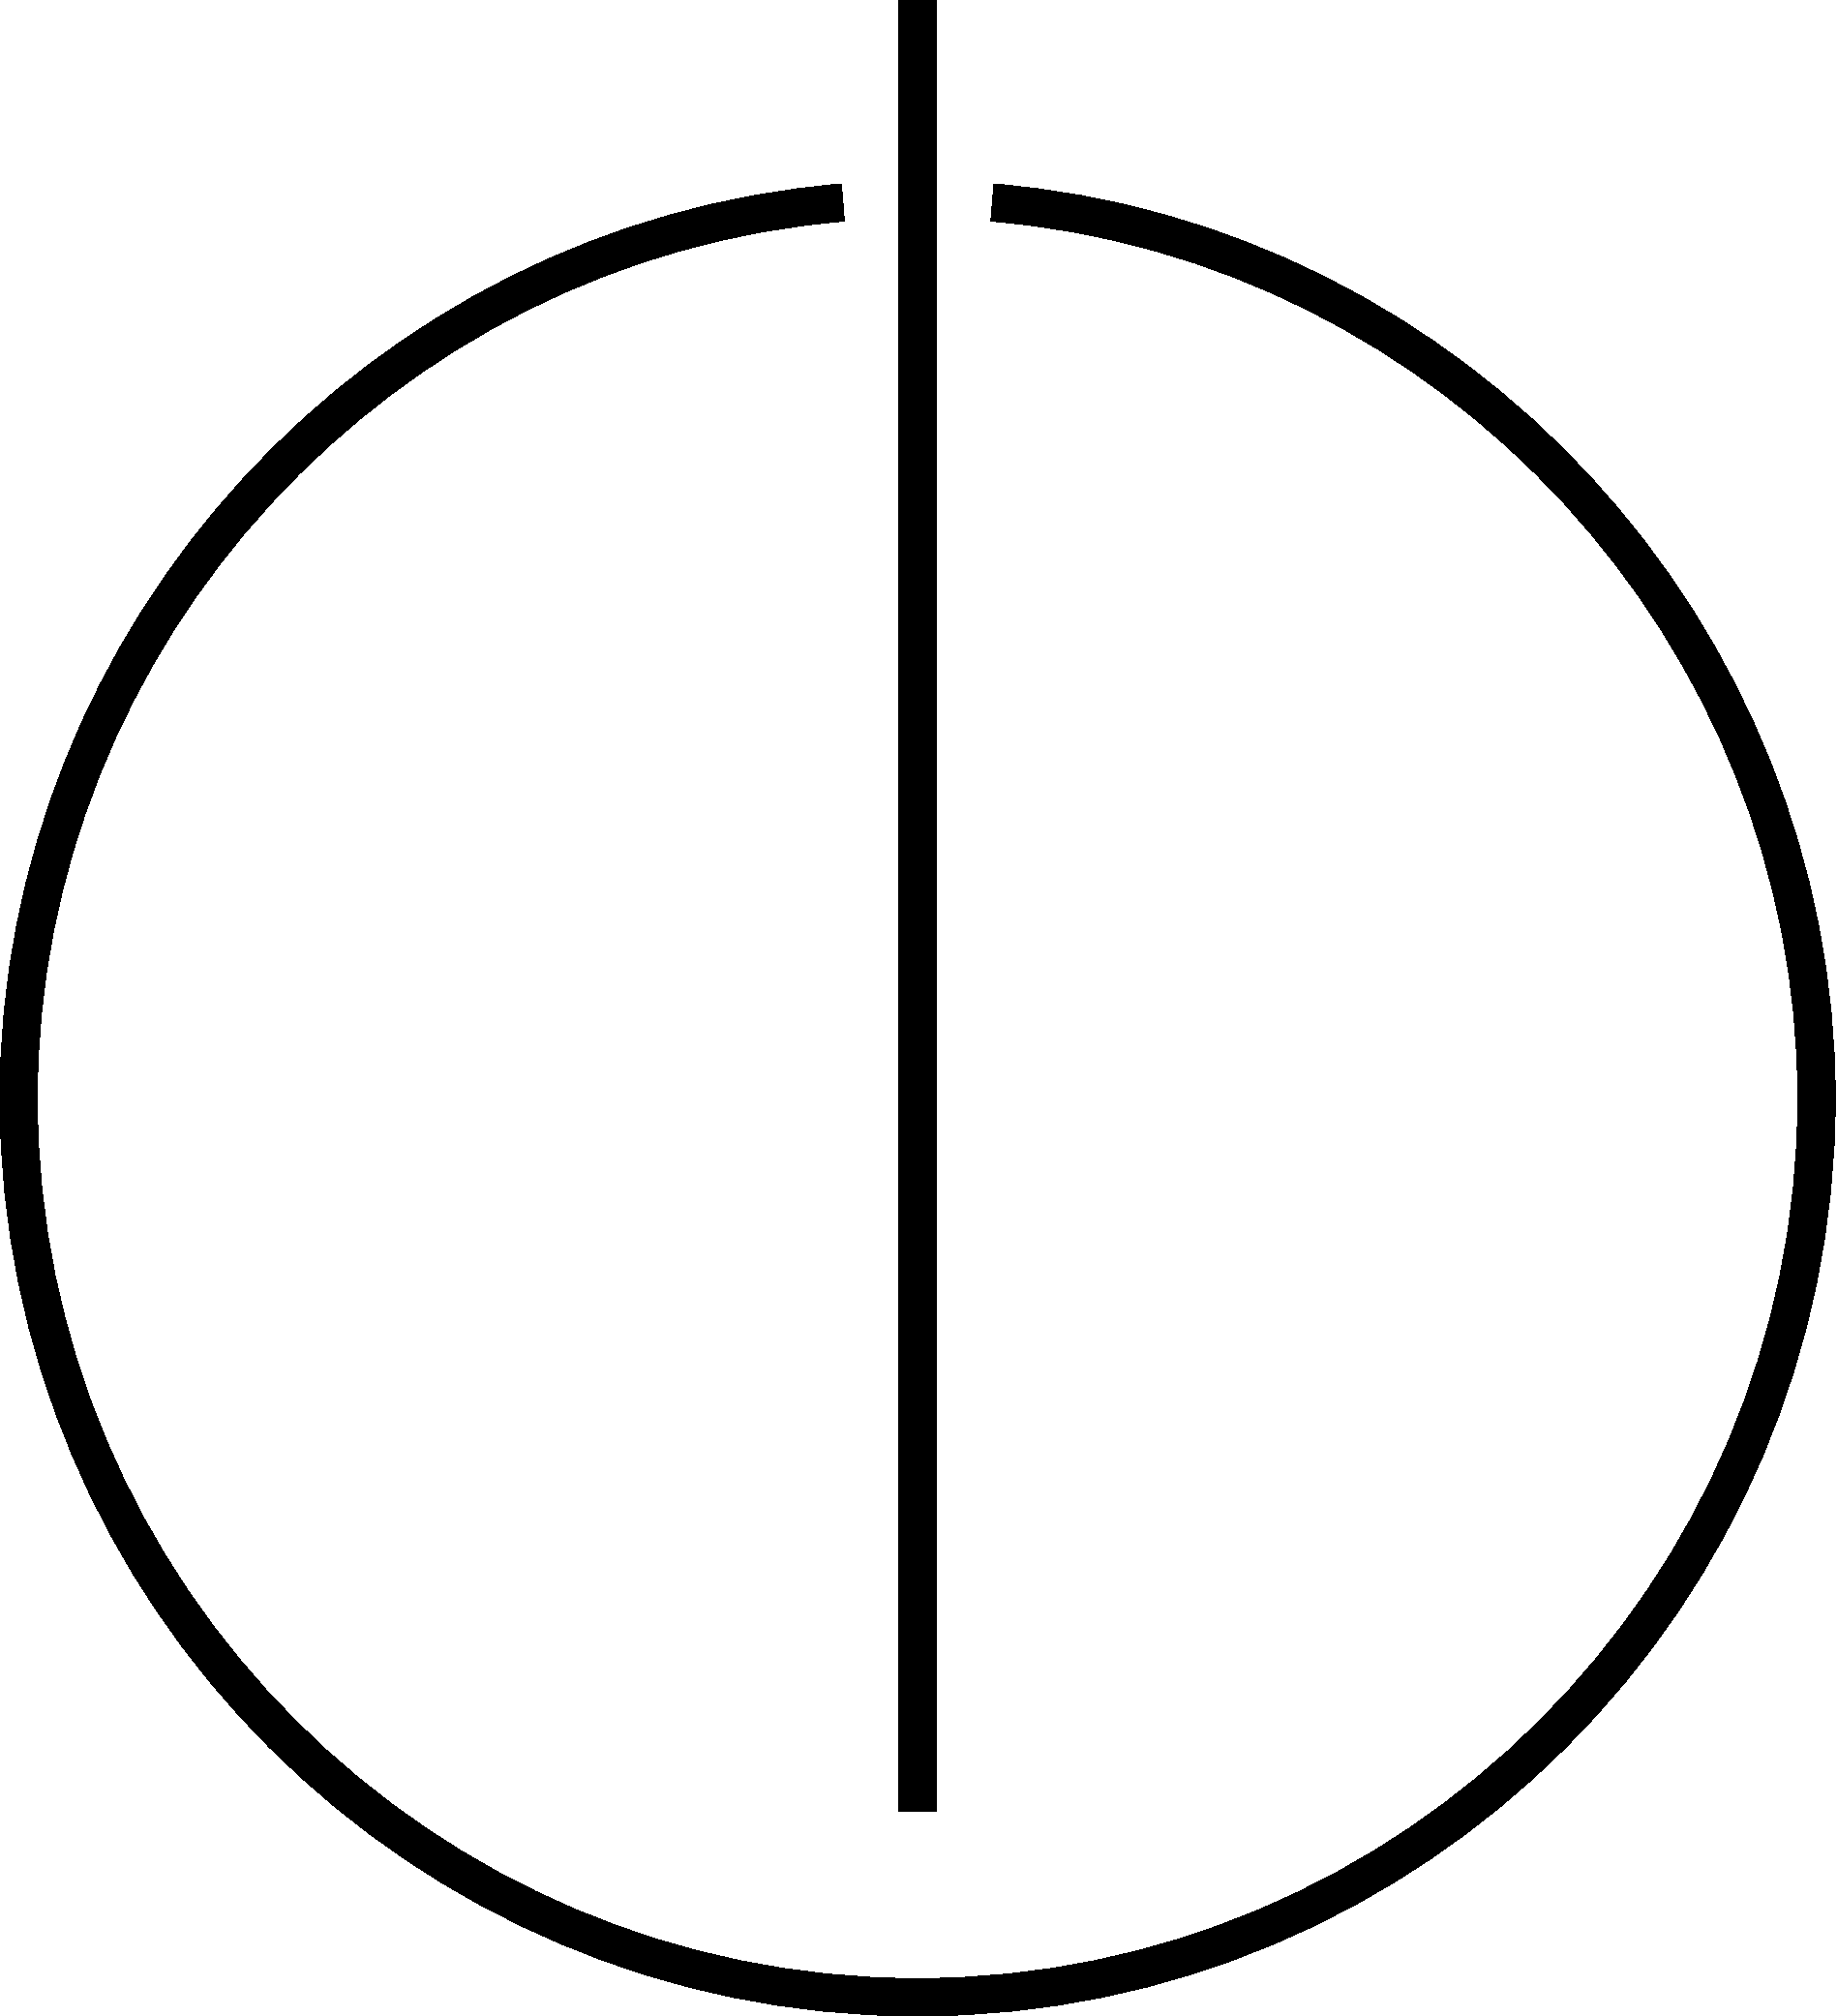
\includegraphics[height=20mm]{thesis/logos/faculty.pdf}
  }{}
\end{titlepage}
\cleardoublepage{}

\thispagestyle{empty}
\vspace*{0.8\textheight}
\noindent
I confirm that this bachelor's thesis is my own work and I have documented all sources and material used.

\vspace{15mm}
\noindent
\getSubmissionLocation{}, \getSubmissionDate{} \hspace{50mm} \getAuthor{}

\cleardoublepage{}

\addcontentsline{toc}{chapter}{Acknowledgments}
\thispagestyle{empty}

\vspace*{20mm}

\begin{center}
{\usekomafont{section} Acknowledgments}
\end{center}

\vspace{10mm}

%TODO: Acknowledgments

\cleardoublepage{}

\chapter{\abstractname}

The energy consumption of data centers assumes a significant fraction of the worlds overall energy consumption. Most data centers are statically provisioned leading to a very low average utilization of servers. In this work we survey uni-dimensional and high-dimensional approaches for dynamically powering-up and powering-down servers to reduce the energy footprint of data centers while ensuring that incoming jobs are processed in-time. We implement algorithms for smoothed online convex optimization and variations thereof where in each round the agent receives a convex cost function. The agent seeks to minimize cost based on an exploration-exploitation trade-off using an additional switching cost which is associated with changing decisions in-between rounds. We implement the algorithms in their most general form, inviting future research on their performance in other application areas. We evaluate the algorithms for the application of right-sizing data centers using traces from Facebook, Microsoft, Alibaba, and Los Alamos National Lab. Our experiments show that the the online algorithms perform close to the dynamic offline optimum in practice and promise a significant cost reduction when compared to the static offline optimum. We discuss how features of the data center model and trace impact the performance. Finally, we investigate the practical use of predictions to achieve further cost reductions.

\microtypesetup{protrusion=false}
\tableofcontents{}
\microtypesetup{protrusion=true}

\mainmatter{}

% !TeX root = ../main.tex
% Add the above to each chapter to make compiling the PDF easier in some editors.

\chapter{Introduction}\label{chapter:introduction}

\section{Section}
Citation test~\parencite{latex}.

\subsection{Subsection}

See~\autoref{tab:sample}, \autoref{fig:sample-drawing}, \autoref{fig:sample-plot}, \autoref{fig:sample-listing}.

\begin{table}[htpb]
  \caption[Example table]{An example for a simple table.}\label{tab:sample}
  \centering
  \begin{tabular}{l l l l}
    \toprule
      A & B & C & D \\
    \midrule
      1 & 2 & 1 & 2 \\
      2 & 3 & 2 & 3 \\
    \bottomrule
  \end{tabular}
\end{table}

\begin{figure}[htpb]
  \centering
  % This should probably go into a file in figures/
  \begin{tikzpicture}[node distance=3cm]
    \node (R0) {$R_1$};
    \node (R1) [right of=R0] {$R_2$};
    \node (R2) [below of=R1] {$R_4$};
    \node (R3) [below of=R0] {$R_3$};
    \node (R4) [right of=R1] {$R_5$};

    \path[every node]
      (R0) edge (R1)
      (R0) edge (R3)
      (R3) edge (R2)
      (R2) edge (R1)
      (R1) edge (R4);
  \end{tikzpicture}
  \caption[Example drawing]{An example for a simple drawing.}\label{fig:sample-drawing}
\end{figure}

\begin{figure}[htpb]
  \centering

  \pgfplotstableset{col sep=&, row sep=\\}
  % This should probably go into a file in data/
  \pgfplotstableread{
    a & b    \\
    1 & 1000 \\
    2 & 1500 \\
    3 & 1600 \\
  }\exampleA
  \pgfplotstableread{
    a & b    \\
    1 & 1200 \\
    2 & 800 \\
    3 & 1400 \\
  }\exampleB
  % This should probably go into a file in figures/
  \begin{tikzpicture}
    \begin{axis}[
        ymin=0,
        legend style={legend pos=south east},
        grid,
        thick,
        ylabel=Y,
        xlabel=X
      ]
      \addplot table[x=a, y=b]{\exampleA};
      \addlegendentry{Example A};
      \addplot table[x=a, y=b]{\exampleB};
      \addlegendentry{Example B};
    \end{axis}
  \end{tikzpicture}
  \caption[Example plot]{An example for a simple plot.}\label{fig:sample-plot}
\end{figure}

\begin{figure}[htpb]
  \centering
  \begin{tabular}{c}
  \begin{lstlisting}[language=SQL]
    SELECT * FROM tbl WHERE tbl.str = "str"
  \end{lstlisting}
  \end{tabular}
  \caption[Example listing]{An example for a source code listing.}\label{fig:sample-listing}
\end{figure}

% !TeX root = ../main.tex
% Add the above to each chapter to make compiling the PDF easier in some editors.

\chapter{Theory}\label{chapter:theory}

\section{Problems}

\subsection{Smoothed Convex Optimization}

\begin{problem}[Smoothed Convex Optimization (SCO)]
Given a time horizon $T \in \mathbb{N}$, a convex decision space $\mathcal{X} \subset \mathbb{R}^d$, a norm $\norm{\cdot}$ on $\mathbb{R}^d$, and a sequence of non-negative convex functions $f_t$ for $t \in [T]$ with $f_t(x) = \infty$ for all $x \not\in \mathcal{X}$, find $x \in \mathcal{X}$ minimizing \begin{align*}
    c(x) = \sum_{t=1}^T f_t(x_t) + \norm{x_t - x_{t-1}}
\end{align*}
where $x_0 = 0$.
\end{problem}

In many practical applications of Smoothed Convex Optimization, we seek to find integral solutions minimizing hitting and switching costs. This is especially true within the context of resource allocation, for example for right-sizing data centers, where our resources are discrete. This observation motivates the definition of the following variant of SCO.

\begin{problem}[Integral Smoothed Convex Optimization (Int-SCO)]
We define Integral Smoothed Convex Optimization analogously to SCO with the added restriction that the points $x$ in $d$-dimensional space must be discrete, that is $\mathcal{X} \subset \mathbb{Z}^d$.
\end{problem}

\subsubsection{Complexity of the Offline Problem}

We now want to examine the complexity of Int-SCO in the offline case. That is, we know all arriving convex cost functions $f_t$ in advance. We prove Int-SCO NP-hard for varying $d$ by giving a polynomial-time reduction from the Knapsack problem. In \autoref{section:theory:simplified_smoothed_convex_optimization} we first extend this proof of NP-hardness to the Integral Simplified Smoothed Convex Optimization problem which restricts the decision space and switching cost. Then, in \autoref{section:theory:smoothed_balanced_load_optimization}, we extend the proof to the Integral Smoothed Balanced-Load Optimization problem which further restricts the structure of the cost functions.

Given a set of items with an associated value and weight and an upper bound to the total weight, Knapsack is the problem of determining the number of copies of each item that maximizes the total value and conforms to the given upper bound on total weight. Formally we define Knapsack as follows.

\begin{problem}[Knapsack (KP)]
Given a number of items $n \in \mathbb{N}$, a value of each item $v \in \mathbb{N}^n$, a weight of each item $w \in \mathbb{N}^n$, and an upper bound to the total weight $W \in \mathbb{N}$, find $x \in \{0,1\}^n$ satisfying $\sum_{i = 1}^n w_i x_i \leq W$ and maximizing $\sum_{i=1}^n v_i x_i$.
is maximized.
\end{problem}

This variant of Knapsack is commonly called \textit{0-1 Knapsack} and restricts the number of copies of each item to be either 0 or 1. It is, however, easy to see that our proof can easily be generalized to a setting where we allow $x_i \in [m_i]_0$ for $m \in \mathbb{N}^n$. TODO et al. show that the Knapsack decision problem is NP-complete and that the Knapsack optimization problem is NP-hard.

Before reducing to Int-SCO, we reduce Knapsack to a related problem called Minimum Knapsack.

\begin{problem}[Minimum Knapsack (Min-KP)]
Given a number of items $n \in \mathbb{N}$, a cost of each item $c \in \mathbb{N}^n$, a utility of each item $u \in \mathbb{N}^n$, and a lower bound to the total utility $U \in \mathbb{N}$, find $x \in \{0,1\}^n$ satisfying $\sum_{i = 1}^n u_i x_i \geq U$ and minimizing $\sum_{i=1}^n c_i x_i$.
\end{problem}

\begin{lemma}
Min-KP is NP-hard.
\end{lemma}

\begin{proof}
We prove the lemma by giving a reduction from KP.

Let $\mathcal{I}_1 = (n, v, w, W)$ be an instance of KP. Let $\mathcal{I}_2(U) = (n, c, u, U)$ be an instance of Min-KP with $c = w$, and $u = v$. Hence, $\mathcal{I}_2(U)$ minimizes the total weight $\sum_{i=1}^n w_i x_i$ such that $\sum_{i=1}^n v_i x_i \geq U$.

By finding solutions to $\mathcal{I}_2(U)$ repeatedly for varying $U$, we determine the maximal $U$ such that $\sum_{i=1}^n w_i x_i \leq W$. Let $v_{max} = \max\{v_i \mid i \in [n]\}$ be the maximal value of any item. We observe that $U$ is upper bounded by $n \cdot v_{max}$. If $U$ were greater than $n \cdot v_{max}$ we would have $\sum_{i=1}^n v_{max} x_i \geq \sum_{i=1}^n v_i x_i > n \cdot v_{max}$ which contradicts $x \in \{0,1\}^n$. Hence, we can use binary search to find $U$ in $\mathcal{O}(\log n + \log v_{max})$ iterations. The other direction works analogously.

We have seen a total, polynomial-time reduction from KP to Min-KP. Hence, Min-KP is NP-hard.
\end{proof}

Next we prove our main reduction from Min-KP to Int-SCO. To motivate this reduction, we first prove that the following (convex) integer optimization is in fact equivalent to Min-KP.

\begin{lemma}
\label{lemma:integer_minimization}
Let $\mathcal{I} = (n, c, u, U)$ be an instance of Min-KP. $x$ is the solution to $\mathcal{I}$ if and only if $x$ minimizes \begin{align*}
    c'(x) = \sum_{i=1}^n c_i x_i + M(U - \sum_{i=1}^n u_i x_i)^+
\end{align*} subject to $x \in \{0,1\}^n$ for some $M > \frac{c_{max}}{u_{min}}$.
\end{lemma}

\begin{proof}
Suppose $x$ minimizes $c'(x)$. Now suppose $(U - \sum_{i=1}^n u_i x_i)^+ > 0$. Then, $(U - \sum_{i=1}^n u_i x_i)^+ \geq u_{min}$. Therefore, $c'(x) > \sum_{i=1}^n c_i x_i + c_{max}$. We observe that $x$ is not optimal as either $c'(x)$ could be minimized further by increasing $x$ such that $(U - \sum_{i=1}^n u_i x_i)^+ = 0$ since $\sum_{i=1}^n c_i x_i \leq c_{max}$ holds for all $x$. Alternatively, $x$ already equals 1 in each dimension in which case $\sum_{i=1}^n u_i < U$, indicating that $\mathcal{I}$ has no solution.

By leading our previous assumption to a contradiction, we conclude $(U - \sum_{i=1}^n u_i x_i)^+ = 0$ and therefore $U \leq \sum_{i=1}^n u_i x_i$. Further, $c'(x)$ minimizes $\sum_{i=1}^n c_i x_i$ for all remaining candidates for $x$. Hence, $x$ is the solution of $\mathcal{I}$.

On the other hand, suppose that $x$ is the solution to $\mathcal{I}$. Then $(U - \sum_{i=1}^n u_i x_i)^+ = 0$ and $\sum_{i=1}^n c_i x_i$ is minimized. Hence, $x$ minimizes $c'(x)$.
\end{proof}

For our construction we need that $c$ is convex.

\begin{lemma}
\label{lemma:integer_minimization_convexity}
$c'(\cdot)$ is convex.
\end{lemma}

\begin{proof}
It is easy to see that $c$ is continuous. Therefore, to show the convexity of $c$ it suffices to prove $c'(\frac{x+y}{2}) \leq \frac{c'(x)+c'(y)}{2}$ for all $x, y \in \mathbb{R}^n$.

To simplify the notation let $c'(x) = \sum_{i=1}^n c_i x_i$ and let $U(x) = \sum_{i=1}^n u_i x_i$. To further simplify the notation we define $\frac{x+y}{2}$ to be applied component-wise to elements $i \in [n]$ of $x$ and $y$. We then obtain \small{
\begin{align*}
         &c'(\frac{x+y}{2}) \leq \frac{c'(x)+c'(y)}{2} \\
    \iff &C(\frac{x+y}{2}) + M(U - U(\frac{x+y}{2}))^+ \leq \frac{C(x) + M(U - U(x))^+ + C(y) + M(U - U(y))^+}{2} \\
    \iff &C(x) + C(y) + 2M(U - U(\frac{x+y}{2}))^+ \leq C(x) + M(U - U(x))^+ + C(y) + M(U - U(y))^+ \\
    \iff &2(U - U(\frac{x+y}{2}))^+ \leq (U - U(x))^+ + (U - U(y))^+.
\end{align*}
}\normalsize

We immediately get the convexity of $U(\cdot)$ by the following equivalence. \begin{align*}
    U(\frac{x+y}{2}) &= \sum_{i=1}^n u_i \frac{x_i + y_i}{2} \\
                     &= \frac{\sum_{i=1}^n u_i x_i + \sum_{i=1}^n u_i y_i}{2} \\
                     &= \frac{U(x) + U(y)}{2}.
\end{align*}

Now, we consider three cases separately.

\begin{enumerate}
    \item If $U(x) > U$ and $U(y) > U$, then $U(\frac{x+y}{2}) > U$. Hence \begin{align*}
        2(U - U(\frac{x+y}{2}))^+ = 0 = (U - U(x))^+ + (U - U(y))^+.
    \end{align*}
    \item If $U(x) \leq U$ and $U(y) \leq U$, then $U(\frac{x+y}{2}) \leq U$. Hence \begin{align*}
        2(U - U(\frac{x+y}{2}))^+ &= 2U - 2U(\frac{x+y}{2}) \\
                                  &= 2U - U(x) + U(y) \\
                                  &= (U - U(x))^+ + (U - U(y))^+.
    \end{align*}
    \item For the only remaining case we assume w.l.o.g. that $U(x) \leq U$ and $U(y) > U$. If $U - U(x) < U(y) - U$, then $U(\frac{x+y}{2}) > U$ and we follow the first case. If, on the other hand, $U - U(x) \geq U(y) - U$, then $U(\frac{x+y}{2}) \leq U$ and we follow the second case.\qedhere
\end{enumerate}
\end{proof}

We now have everything in place to prove our main result of this section.

\begin{theorem}
Int-SCO is NP-hard.
\end{theorem}

\begin{proof}
We now give our reduction from Min-KP to Int-SCO.

Let $\mathcal{I}_1 = (n, c, u, U)$ be an instance of Min-KP. We define $\mathcal{I}_2 = (T, \mathcal{X}, \norm{\cdot}, f)$ as an instance of Int-SCO with $T = 1$, $\mathcal{X} = \{0,1\}^n$, $\norm{\cdot} = 0$, and $f_1(x) = c'(x)$. We further set $d = n$. By \autoref{lemma:integer_minimization_convexity}, $\mathcal{I}_2$ is a valid instance of Int-SCO.

The correctness of our construction follows from \autoref{lemma:integer_minimization}.

\begin{align*}
         &x \text{ is a solution to } \mathcal{I}_2 \\
    \iff &x \text{ minimizes } \sum_{t=1}^T f_t(x_t) + \norm{x_t - x_{t-1}} \text{ such that } x_t \in \mathcal{X}. \\
    \iff &x \text{ minimizes } c'(x_1) \text{ such that } x_1 \in \{0,1\}^n. \\
    \iff &x_1 \text{ is a solution to } \mathcal{I}_1.
\end{align*}

Our construction is total and polynomial in the size of $\mathcal{I}_1$. Hence, Int-SCO is NP-hard.
\end{proof}

We observe that the above reduction can be extended to Knapsack with arbitrary bounds $m_i$ by setting $\mathcal{X}$ of $\mathcal{I}_2$ to $[m_1]_0 \times \dots \times [m_n]_0$.

\subsection{Simplified Smoothed Convex Optimization}
\label{section:theory:simplified_smoothed_convex_optimization}

In many applications, for example for right-sizing data centers, it suffices to restrict $\mathcal{X}$ to $\mathcal{X} = [m_0]_0 \times \dots \times [m_d]_0$ for some $m \in \mathbb{N}^d$ and the switching cost $\norm{x}$ to $\sum_{k=1}^d \beta_k x_k^+$ where $\beta$ is constant for each dimension. To that end, we first define a restricted variant of (fractional) SCO which we term \textit{Simplified Smoothed Convex Optimization}.

\begin{problem}[Simplified Smoothed Convex Optimization (SSCO)]
Given a time horizon $T \in \mathbb{N}$, upper bounds $m \in \mathbb{N}^d$, switching costs $\beta \in \mathbb{R}_{>0}^d$, and a sequence of non-negative convex functions $f_t$ for $t \in [T]$, find $x \in \mathbb{R}_{\geq 0, \leq m_0} \times \dots \times \mathbb{R}_{\geq 0, \leq m_d}$ minimizing \begin{align*}
    c(x) = \sum_{t=1}^T f_t(x_t) + \sum_{k=1}^d \beta_k (x_{t,k} - x_{t-1,k})^+
\end{align*}
where $x_0 = 0$.
\end{problem}

We observe that $c(\cdot)$ pays the switching cost whenever $x$ increases. Decreasing $x$ does not increase the paid switching cost. This observation indicates that the following cost function $d(\cdot)$ is equivalent to $c(\cdot)$.

\begin{definition}[Inverted Simplified Smoothed Convex Optimization]
\begin{align*}
    d(x) = \sum_{t=1}^T f_t(x_t) + \sum_{k=1}^d \beta_k (x_{t,k} - x_{t+1,k})^+.
\end{align*}
Instead of $x_0 = 0$ we require $x_{T+1} = 0$.
\end{definition}

With the same motivation we used for the restriction of SCO to Int-SCO, we now restrict SSCO to an integral variant.

\begin{problem}[Integral Simplified Smoothed Convex Optimization (Int-SSCO)]
We define Integral Simplified Smoothed Convex Optimization analogously to SSCO with the added restriction that the points $x$ in $d$-dimensional space must be discrete, that is $x \in [m_0]_0 \times \dots \times [m_d]_0$.
\end{problem}

\subsubsection{Complexity of the Offline Problem}

We next extend our proof of NP-hardness of Int-SCO for varying $d$ to Int-SSCO. We cannot reuse our original proof as the switching cost of SSCO is required to be positive.

\subsection{Smoothed Balanced-Load Optimization}
\label{section:theory:smoothed_balanced_load_optimization}

\subsection{Smoothed Load Optimization}

\subsubsection{Complexity of the Offline Problem}

\section{Algorithm Analysis}

\subsection{Approximations}

\subsection{Regret}

\subsection{Competitiveness}

% !TeX root = ../main.tex
% Add the above to each chapter to make compiling the PDF easier in some editors.

\chapter{Application: Right-Sizing Data Centers}\label{chapter:application_data_centers}

\section{Server Infrastructures}

\section{Modeling Cost}

\subsection{Optimal Load Balancing}

\section{Modeling Time}

\section{Using Online Algorithms in Practice}

% !TeX root = ../main.tex
% Add the above to each chapter to make compiling the PDF easier in some editors.

\chapter{Offline Algorithms}\label{chapter:algorithms}

\section{Uni-Dimensional}

\subsection{Capacity Provisioning}

\subsubsection{Backward-Recurrent}

\subsubsection{Forward-Recurrent}

\subsection{Graph-Based Optimal Discrete Algorithm}

\subsection{[Graph-Based Linear-Time Discrete Approximation Algorithm]}

\section{Multi-Dimensional}

\subsection{[Optimal Continuous Algorithm]}

\subsection{Graph-Based Optimal Discrete Algorithm}

\subsection{Graph-Based Polynomial-Time Discrete Approximation Algorithm}

% !TeX root = ../main.tex
% Add the above to each chapter to make compiling the PDF easier in some editors.

\chapter{Online Algorithms}\label{chapter:online_algorithms}

In this chapter, we discuss the online algorithms we implemented in our work. Similarly, to the previous chapter on offline algorithms, we begin our discussion in \autoref{section:online_algorithms:ud} with algorithms for the uni-dimensional setting. As was discussed in \autoref{chapter:theory}, these algorithms give strong guarantees yielding a constant competitive ratio. Next in \autoref{section:online_algorithms:md}, we extend our discussion to the multi-dimensional setting. Here, the guarantees are not as strong. We thus begin in \autoref{section:online_algorithms:md:lazy_budgeting} by considering lazy budgeting algorithms for smoothed convex optimization problems with very specific cost functions. As mentioned previously in \autoref{chapter:theory}, while there are algorithms with sublinear regret (gradient descent) there cannot be any algorithms achieving a dimension-independent constant competitive ratio unless the class of allowed cost functions is restricted \cite{Chen2018}. In \autoref{section:online_algorithms:md:descent_methods}, we therefore discuss gradient methods that have been shown to be able to perform well with regard to either the competitive ratio or regret with a restricted class of cost functions. Still, sublinear regret and a constant competitive ratio cannot be achieved at the same time, even for linear cost functions \cite{Andrew2015}. We therefore end this chapter in \autoref{section:online_algorithms:md:predictions} with a discussion of algorithms that make use of predictions to circumvent this fundamental limitation.

Throughout this chapter, we denote by $\tau \in [T]$ the current time slot. In contrast to offline algorithms that know the hitting costs $f_t$ for all $t \in [T]$, an online algorithm only knows the hitting costs $f_t$ up to $\tau$, i.e. $t \in [\tau]$.

\section{Uni-Dimensional}\label{section:online_algorithms:ud}

\subsection{Lazy Capacity Provisioning}\label{section:online_algorithms:ud:lazy_capacity_provisioning}

\subsubsection{Fractional Algorithm}

We begin by returning to the notion of capacity provisioning that we introduced in \autoref{section:offline_algorithms:ud:capacity_provisioning} yielding a backward-recurrent algorithm finding an optimal schedule for SSCO. This algorithm computed bounds $X_{\tau}^L$ and $X_{\tau}^U$ on the optimal solution which only depend on the schedule up to time slot $\tau$. However, the optimal offline algorithm stayed within these bounds moving backwards in time which is not possible for an online algorithm. \citeauthor*{Lin2011} present a similar algorithm moving forward in time called \emph{lazy capacity provisioning} \cite{Lin2011}. We computes the schedule $X_{\tau}$ during time slot $\tau$ by setting $X_{\tau} = X_{\tau-1}$ unless this violates the bounds in which case we make the smallest possible change: \begin{align*}
    X_{\tau} = \begin{cases}
        0 & \tau \leq 0 \\
        (X_{\tau-1})_{X_{\tau,\tau}^L}^{X_{\tau,\tau}^U} & \tau \geq 1
    \end{cases}
\end{align*} where $(X_{\tau-1})_{X_{\tau,\tau}^L}^{X_{\tau,\tau}^U}$ is the projection of $X_{\tau-1}$ onto $[X_{\tau,\tau}^L, X_{\tau,\tau}^U]$ \cite{Lin2011}. [TODO: add figure comparing to brcp and link from section on brcp]. The resulting algorithm is described in \autoref{alg:ud:lcp}. Similarly to the offline algorithm, we are able to use algorithms for convex optimization to compute the upper and lower bounds. Hence, we obtain a complexity of $\mathcal{O}(\tau C O_{\epsilon})$ for $\epsilon$-optimal upper and lower bounds. This complexity is worrying as it depends on $\tau$ which may grow to be very large. However, \citeauthor*{Lin2011} prove the following lemma which implies that it suffices to compute the lower and upper bounds using only the history since the last time slot where the bounds were either both decreased or both increased.

\begin{lemma}
If there exists an index $t \in [1, \tau-1]$ such that $X_{\tau,t+1}^U < X_{\tau,t}^U$ or $X_{\tau,t+1}^L > X_{\tau,t}^L$, then $(\hat{X}_{\tau,1},\dots,\hat{X}_{\tau,t}) := (X_{\tau,1}^L,\dots,X_{\tau,t}^L) = (X_{\tau,1}^U,\dots,X_{\tau,t}^U)$, and no matter what the future arrival is, solving the optimization in $[1,\tau']$ for $\tau' > \tau$ is equivalent to solving two optimizations: one over $[1,t]$ with initial condition $X_0$ and final condition $\hat{X}_{\tau,t}$ and the second over $[t+1,\tau']$ with initial condition $\hat{X}_{\tau,t}$ \cite{Lin2011}.
\end{lemma}

While not changing the worst-case complexity, this significantly improves the practical complexity in the application of right-sizing data centers as diurnal load patterns typically ensure that less than a day needs to be considered \cite{Lin2011}. We denote by $X_{\tau}^{L,(t,x_0)}$ and $X_{\tau}^{U,(t,x_0)}$ the bounds resulting from optimizations beginning at time slot $t$ with initial condition $x_0$. \citeauthor*{Lin2011} showed that lazy capacity provisioning is tightly $3$-competitive \cite{Lin2011}.

\begin{algorithm}
    \caption{Lazy Capacity Provisioning \cite{Lin2011}}\label{alg:ud:lcp}
    \SetKwInOut{Input}{Input}
    \Input{$\mathcal{I}_{\text{SSCO}} = (\tau \in \mathbb{N}, m \in \mathbb{N}, \beta \in \mathbb{R}_{>0}, (f_1, \dots, f_{\tau}) \in (\mathbb{R}_{\geq 0} \to \mathbb{R}_{\geq 0})^{\tau})$}
    $t_0 \gets 0$\;
    $x_0 \gets 0$\;
    \For{$t \gets \tau-1$ \KwTo $2$}{
        \If{$X_{t,t}^U < X_{t,t-1}^U \lor X_{t,t}^L > X_{t,t-1}^L$}{
            $t_0 \gets t$\;
            $x_0 \gets X_{t,t-1}^U$\;
            \KwBreak
        }
    }
    \Return $(X_{\tau-1})_{X_{\tau,\tau}^{L,(t_0,x_0)}}^{X_{\tau,\tau}^{U,(t_0,x_0)}}$\;
\end{algorithm}

\subsubsection{Integral Algorithm}

\citeauthor*{Albers2018} applied lazy capacity provisioning to the integral variant Int-SSCO using their graph-based offline algorithm discussed in \autoref{section:offline_algorithms:ud:graph_based} to compute the integral lower and upper bounds \cite{Albers2018}. It is apparent, that this immediately yields a deterministic online algorithm for Int-SSCO. \citeauthor*{Albers2018} showed that similar to lazy capacity provisioning their algorithm is $3$-competitive \cite{Albers2018}. Due to the changed method of determining the bounds its runtime is $\mathcal{O}(\tau C \log_2 m)$. By using the same method of shortening the used history that was proposed by \citeauthor*{Lin2011} we are able to reduce this time complexity drastically in practice (for large $\tau$). Thus, the adopted algorithm is still described by \autoref{alg:ud:lcp}. We simply need to slightly modify the graph-based algorithm computing optimal offline solutions to allow for initial conditions other than $0$.

\subsection{Memoryless Algorithm}

\citeauthor*{Bansal2015} showed that for SSCO a competitive ratio of $3$ can also be attained by a memoryless algorithm \cite{Bansal2015}. In a memoryless online algorithm for smoothed convex optimization, the configuration $X_{\tau}$ only depends on the preceding configuration $X_{\tau-1}$ and the current hitting cost $f_{\tau}$. This generally allows for a more space and time efficient algorithm. This is important when we want to choose a small time slot length $\delta$ so as to be more responsive to changes in load.

The algorithm proposed by \citeauthor*{Bansal2015} works as follows. Let $x_m$ be the minimizer of $f_{\tau}(x)$, i.e. $x_m = \argmin_{x \in \mathcal{X}} f_{\tau}(x)$. The algorithm moves into the direction of the minimizer until it either reaches $x_m$, or it reaches a configuration $x$ where its switching cost equals twice the hitting cost of $x$. [TODO: add figure depicting search space of convex optimization]. We observe that this is equivalent to the following convex optimization: \begin{align}\label{eq:ud:memoryless}\begin{aligned}
    &\min_{x \in \mathcal{X}} &&f_{\tau}(x) \\
    &\text{subject to}        &&|x - X_{\tau-1}| \leq \frac{f_{\tau}(x)}{2}.
\end{aligned}\end{align} The resulting algorithm is simply given by determining $\hat{x}$ based on the convex optimization in \autoref{eq:ud:memoryless}, see \autoref{alg:ud:memoryless}. Thus, the time (and space) complexity of this memoryless algorithm is $\mathcal{O}(C O_{\epsilon})$ for finding $\epsilon$-optimal solutions.

\begin{algorithm}
    \caption{Memoryless algorithm \cite{Bansal2015}}\label{alg:ud:memoryless}
    \SetKwInOut{Input}{Input}
    \Input{$\mathcal{I}_{\text{SSCO}} = (\tau \in \mathbb{N}, m \in \mathbb{N}, \beta \in \mathbb{R}_{>0}, (f_1, \dots, f_{\tau}) \in (\mathbb{R}_{\geq 0} \to \mathbb{R}_{\geq 0})^{\tau})$}
    \Return $\hat{x}$ such that that $\hat{x}$ is the result of the optimization in \autoref{eq:ud:memoryless}\;
\end{algorithm}

\subsection{Probabilistic Algorithm}\label{section:online_algorithms:ud:probabilistic}

Next, we discuss a $2$-competitive algorithm developed by \citeauthor*{Bansal2015} which works by maintaining a probability distribution over configurations \cite{Bansal2015}. Using this probability distribution they describe a randomized algorithm which they subsequently translate into a deterministic algorithm. We begin our description by describing how to gather first a randomized and then a deterministic algorithm from a probability distribution. Then, we describe how \citeauthor*{Bansal2015} determine the probability distribution and how it can be computed in practice.

\subsubsection{From Probability Distribution to Deterministic Algorithm}

Let's suppose we have given a probability distribution $p$ over configurations $x \in \mathcal{X}$. A randomized algorithm is then described by initially picking a number $\gamma \in [0,1]$ uniformly at random and then maintaining the invariant that at time $\tau$ the chosen configuration $x_{\tau}$ has the property that the probability mass to the left of $x_{\tau}$ with respect to $p$ is exactly $\gamma$ \cite{Bansal2015}. Crucially, this approach only works in the fractional setting. Also note that $\gamma$ is chosen only once prior to running the algorithm. This describes how we obtain a randomized algorithm from a probability distribution over configurations.

Next, \citeauthor*{Bansal2015} show the following theorem which describes how we can obtain a deterministic algorithm from a randomized algorithm. \begin{theorem}
    For the problem of (fractional) online convex optimization, if there exists a $\rho$-competitive randomized algorithm $\mathcal{R}$ then there exists a $\rho$-competitive deterministic algorithm $\mathcal{D}$ \cite{Bansal2015}.
\end{theorem}
\begin{proof}
\citeauthor*{Bansal2015} prove this theorem using Jensen's inequality. In the setting of a probability space, \textit{Jensen's inequality}\index{Jensen's inequality} claims that given a convex function $\varphi$ and a random variable $X$ we have \begin{align}
    E(\varphi(X)) \geq \varphi(E X)
\end{align} provided both expectations exist, i.e. $E |X|$ and $E |\varphi(X)| < \infty$ \cite{Durrett2010}.

Let $X_{\tau}$ be a random variable denoting the configuration of the randomized algorithm $\mathcal{R}$ at time $\tau$. Then, the deterministic algorithm $\mathcal{D}$ of \citeauthor*{Bansal2015} sets their configuration to $x_{\tau} = E X_{\tau}$. The cost of $\mathcal{D}$ is then given by $f_{\tau}(x_{\tau}) + (x_{\tau} - x_{\tau-1})^+$ and the cost of $\mathcal{R}$ is given by $E(f_{\tau}(X_{\tau})) + E((X_{\tau} - X_{\tau-1})^+)$. We observe that both $f_{\tau}$ and $(\cdot)^+$ are convex functions, implying that the cost of $\mathcal{R}$ is at least $f_{\tau}(E X_{\tau}) + (E X_{\tau} - E X_{\tau-1})^+$ which equals the cost of $\mathcal{D}$. Summing over all $t$ completes the proof \cite{Bansal2015}.
\end{proof}

Hence, we have seen that a deterministic algorithm can be obtained from a randomized algorithm by, in each time slot, choosing the expected configuration of the randomized algorithm. [TODO: add figure depicting probability distribution].

\subsubsection{The Probability Distribution}

For the description of this algorithm we assume that $f_{\tau}$ has well defined first and second order derivatives. Further, we assume that the minimizer $x_m$ of $f_{\tau}$ is unique and bounded. In \autoref{section:theory:beyond_convexity}, we discussed the assumption of differentiability and how it relates to our data center model. The second assumption, namely that the minimizer of the hitting cost, is natural in the setting of a data center as revenue loss increases for small configurations whereas energy costs increase for large configurations. \citeauthor*{Bansal2015} describe how these assumptions can be discharged, but this prohibits a general implementation of the algorithm for arbitrary convex cost functions as the specific shape of the cost function needs to be taken into account \cite{Bansal2015}.

For any time $\tau$, the algorithm maintains a probability distribution $p_{\tau}$ over configurations $x \in \mathcal{X}$. So $\int_a^b p_{\tau}(x) \,dx$ represents the probability that $X_{\tau} \in [a,b]$ for any two $a, b \in \mathcal{X}$. At each time step $\tau$ we first find the minimizer of $f_{\tau}$, $x_m = \argmin_{x \in \mathcal{X}} f_{\tau}(x)$. Then, we find a point $x_r \geq x_m$ such that \begin{align}\label{eq:ud:probabilistic:right}
    \frac{1}{2} \int_{x_m}^{x_r} \diff[2]{f_{\tau}}{y}(y) \,dy = \int_{x_r}^{\infty} p_{\tau-1}(y) \,dy
\end{align} and a point $x_l \leq x_m$ such that \begin{align}\label{eq:ud:probabilistic:left}
    \frac{1}{2} \int_{x_l}^{x_m} \diff[2]{f_{\tau}}{y}(y) \,dy = \int_{-\infty}^{x_l} p_{\tau-1}(y) \,dy.
\end{align} We then update the probability distribution as follows: \begin{align}\label{eq:ud:probabilistic:update}
    p_{\tau}(x) = \begin{cases}
        p_{\tau-1}(x) + \frac{1}{2} \diff[2]{f_{\tau}}{x}(x) & x \in [x_l,x_r] \\
        0 & \text{otherwise}
    \end{cases}
\end{align} where $p_0$ assigns all probability mass to the configuration $0$, i.e. $p_0 = \delta$ where \begin{align*}
    \delta(x) = \begin{cases}
        \infty & x = 0 \\
        0 & x \neq 0
    \end{cases}
\end{align*} is the \textit{Dirac delta function}\index{Dirac delta function} used as a generalized probability density function \cite{Salasnich2015}.

\subsubsection{The Algorithm}

We observe that, using the fundamental theorem of calculus, $x_r$ constrained by \autoref{eq:ud:probabilistic:right} can be found with the following optimization: \begin{align}\label{eq:ud:probabilistic:right:opt}\begin{aligned}
    &\max_{x \in \mathcal{X}} &&x \\
    &\text{subject to}        &&\frac{1}{2} \left(\diff{f_{\tau}}{x}(x) - \diff{f_{\tau}}{x}(x_m)\right) = \int_{x}^{\infty} p_{\tau-1}(y) \,dy \\
    &                         &&x \geq x_m.
\end{aligned}\end{align} Let the above constraint be represented by $g(x) = h(x)$. It is easy to see that $g$ is monotonically increasing as the first order derivative of the convex function $f_{\tau}$ is monotonically increasing and $x \geq x_m$. Moreover, $h$ is monotonically decreasing as it is the negative of the cumulative distribution function of the probability distribution $p_{\tau-1}$. Hence, $g(x) - h(x)$ is monotonically increasing and as such convex. Thus, the optimization described in \autoref{eq:ud:probabilistic:right:opt} is convex.

With a similar argument we are able to determine $x_l$ constrained by \autoref{eq:ud:probabilistic:left} using the optimization: \begin{align}\label{eq:ud:probabilistic:left:opt}\begin{aligned}
    &\min_{x \in \mathcal{X}} &&x \\
    &\text{subject to}        &&\frac{1}{2} \left(\diff{f_{\tau}}{x}(x_m) - \diff{f_{\tau}}{x}(x)\right) = \int_{-\infty}^{x} p_{\tau-1}(y) \,dy \\
    &                         &&x \leq x_m.
\end{aligned}\end{align} Again, let the above constraint be represented by $g(x) = h(x)$. Recall that the first order derivative of $f_{\tau}$ is monotonically increasing. Therefore, $g$ must now be monotonically decreasing as $x_m \geq x$. Further, $h$ is monotonically increasing as it is the cumulative distribution function of the probability distribution $p_{\tau-1}$. Hence, $h(x) - g(x)$ is monotonically increasing and as such convex. This argument shows that also the optimization described in \autoref{eq:ud:probabilistic:left:opt} is convex.

We use the \textit{five-point stencil}\index{five-point stencil} \begin{align*}
    \diff{f_{\tau}}{x}(x) \approx \frac{-f_{\tau}(x - 2h) + 8 f_{\tau}(x + h) - 8 f_{\tau}(x - h) + f_{\tau}(x - 2h)}{12h}
\end{align*} to find a finite difference approximation of order $\mathcal{O}(h)$ of the first order derivative of $f_{\tau}$ at configurations $x \in \mathcal{X}$ \cite{Sauer2011}. To match the accuracy of our convex optimizations we set $h := \epsilon$. To approximate the second order derivative of $f_{\tau}$ at a configuration $x \in \mathcal{X}$ we use \begin{align*}
    \diff[2]{f_{\tau}}{x}(x) \approx \frac{-f_{\tau}(x + 2h) + 16 f_{\tau}(x+h) - 30 f_{\tau}(x) + 16 f_{\tau}(x-h) - f_{\tau}(x - 2h)}{12 h^2}
\end{align*} which yields an approximation of order $\mathcal{O}(h^4)$ \cite{Sauer2011}. Thus, we set $h := \epsilon^{-1/4}$. We are thus able to compute these approximations in $\mathcal{O}(C)$ time.

We use the \textit{double exponential method}\index{double exponential method} (also known as Tanh-sinh quadrature) to compute the integrals over the probability distribution $p$. \citeauthor*{Bailey2005} describe the convergence and error of this method in more detail \cite{Bailey2005}. They conclude that "overall, the tanh-sinh scheme appears to be the best
for integrands of the type most often encountered in experimental math research" and highlight that it has "excellent accuracy and runtime performance" \cite{Bailey2005}. As this integration scheme is not universal, there potentially exist probability distributions for which the double exponential method is unable to find the integral. In such a case one would have to resort to another integration scheme. We denote the convergence rate of approximating the integral with tolerance $\epsilon$ by $\mathcal{O}(I_{\epsilon})$.

Note that the computation of $p_{\tau}$ requires $\mathcal{O}(\tau)$ many approximations of the second order derivative of $f_{t}$. Therefore, any evaluation of $p_{\tau}$ requires $\mathcal{O}(\tau C)$ time and we are thus able to compute the $\epsilon$-optimal integral in $\mathcal{O}(\tau C I_{\epsilon})$ time. Overall, the described convex optimizations can be solved $\epsilon$-optimally in $\mathcal{O}(\tau C I_{\epsilon} O_{\epsilon})$ time. This is also the time complexity of the algorithm. This shows that similarly to lazy capacity provisioning, the computational complexity grows linearly with time. However, unlike for lazy capacity provisioning, we do not have a method of regularly resetting the history, rendering this algorithm computationally inefficient in practice. The algorithm is described in \autoref{alg:ud:probabilistic}.

\begin{algorithm}
    \caption{Probabilistic algorithm \cite{Bansal2015}}\label{alg:ud:probabilistic}
    \SetKwInOut{Input}{Input}
    \Input{$\mathcal{I}_{\text{SSCO}} = (\tau \in \mathbb{N}, m \in \mathbb{N}, \beta \in \mathbb{R}_{>0}, (f_1, \dots, f_{\tau}) \in (\mathbb{R}_{\geq 0} \to \mathbb{R}_{\geq 0})^{\tau})$}
    $x_m \gets \argmin_{x \in \mathcal{X}} f_{\tau}(x)$\;
    find $x_r$ using the optimization described by \autoref{eq:ud:probabilistic:right:opt}\;
    find $x_l$ using the optimization described by \autoref{eq:ud:probabilistic:left:opt}\;
    set $p_{\tau}$ based on the update rule in \autoref{eq:ud:probabilistic:update}\;
    \Return $\int_{x_l}^{x_r} y \cdot p_{\tau}(y) \,dy$\;
\end{algorithm}

Updating the probability distribution $p$ can be done in constant time as this does not require any function evaluations. As discussed in the beginning of this subsection, given a uniformly picked $\gamma \in [0,1]$, the randomized algorithm chooses $X_{\tau}$ (randomly) such that $\int_{-\infty}^{X_{\tau}} p_{\tau}(y) \,dy = \gamma$. In other words, $P_{\tau}(X_{\tau}) \sim \text{Unif}(0,1)$ where $P_{\tau}$ is the cumulative distribution function of $p_{\tau}$. By the universality of the uniform, $X_{\tau}$ is $P_{\tau}$-distributed, i.e. $X_{\tau} \sim P_{\tau}$. Hence, $E X_{\tau} = \int_{x_l}^{x_r} y \cdot p_{\tau}(y) \,dy$ computes the configuration for time slot $\tau$ as $p_{\tau}(y) = 0$ for $y \not\in [x_l, x_r]$. Similarly to the previously discussed integrals, this integral can be computed $\epsilon$-optimally in $\mathcal{O}(\tau C I_{\epsilon})$ time, not affecting the asymptotic time complexity of the algorithm.

\subsection{Randomized Integral Relaxation}

\citeauthor*{Albers2018} use the probabilistic algorithm described in \autoref{section:online_algorithms:ud:probabilistic} in their randomized algorithm for Int-SSCO achieving the optimal competitive ratio $2$ \cite{Albers2018}. Roughly, the algorithm works by solving the relaxed problem using the probabilistic algorithm of \citeauthor*{Bansal2015} and then randomly round the resulting fractional schedule.

Let $\bar{\mathcal{I}}$ be the fractional relaxation of the instance $\mathcal{I}$ of Int-SSCO and let $\bar{\mathcal{X}}$ denote the decision space of $\bar{\mathcal{I}}$. We denote by $\bar{x}_{\tau} \in \bar{\mathcal{X}}$ the configuration at time $\tau$ chosen by \autoref{alg:ud:probabilistic}. Further, let $\text{frac}(x) = x - \lfloor x \rfloor$ be the fractional part of $x$ and let $\bar{x}'_{\tau-1} = (\bar{x}_{\tau-1})_{\lfloor\bar{x}_{\tau}\rfloor}^{\lceil\bar{x}_{\tau}\rceil}$ be the projection of the preceding configuration onto the discrete interval of the current configuration.

The randomized algorithm distinguishes between time slots where the configuration is increased and time slots where the configuration is decreased. In the first case, i.e. $\bar{x}_{\tau-1} \leq \bar{x}_{\tau}$, if $x_{\tau-1} = \lceil\bar{x}_{\tau}\rceil$  the configuration remains unchanged. Otherwise, $x_{\tau}$ is set to $\lceil\bar{x}_{\tau}\rceil$ with probability \begin{align*}
    p_{\tau}^{\uparrow} := \frac{\bar{x}_{\tau} - \bar{x}'_{\tau-1}}{1 - \text{frac}(\bar{x}'_{\tau-1})}
\end{align*} and to $\lfloor\bar{x}_{\tau}\rfloor$ with probability $1 - p_{\tau}^{\uparrow}$. Conversely, if $\bar{x}_{\tau-1} > \bar{x}_{\tau}$, the configuration remains unchanged if $x_{\tau-1} = \lfloor\bar{x}_{\tau}\rfloor$, and otherwise with probability \begin{align*}
    p_{\tau}^{\downarrow} := \frac{\bar{x}'_{\tau-1} - \bar{x}_{\tau}}{\text{frac}(\bar{x}'_{\tau-1})}
\end{align*} the configuration is set to $\lfloor\bar{x}_{\tau}\rfloor$ and with probability $p_{\tau}^{\downarrow}$ the configuration is set to $\lceil\bar{x}_{\tau}\rceil$. The resulting algorithm is shown in \autoref{alg:ud:randomized}.

\begin{algorithm}
    \caption{Randomized integral relaxation \cite{Albers2018}}\label{alg:ud:randomized}
    \SetKwInOut{Input}{Input}
    \Input{$\mathcal{I}_{\text{Int-SSCO}} = (\tau \in \mathbb{N}, m \in \mathbb{N}, \beta \in \mathbb{R}_{>0}, (f_1, \dots, f_{\tau}) \in (\mathbb{N}_0 \to \mathbb{R}_{\geq 0})^{\tau})$}
    $\bar{x}_{\tau} \gets \text{\autoref{alg:ud:probabilistic}}(\bar{\mathcal{I}}_{\text{Int-SSCO}})$\;
    \eIf{$\bar{x}_{\tau-1} \leq \bar{x}_{\tau}$}{
        \eIf{$x_{\tau-1} = \lceil\bar{x}_{\tau}\rceil$}{
            \Return $\lceil\bar{x}_{\tau}\rceil$\;
        }{
            $\gamma \sim \text{Unif}(0,1)$\;
            \eIf{$\gamma \leq p_{\tau}^{\uparrow}$}{
                \Return $\lceil\bar{x}_{\tau}\rceil$\;
            }{
                \Return $\lfloor\bar{x}_{\tau}\rfloor$\;
            }
        }
    }{
        \eIf{$x_{\tau-1} = \lfloor\bar{x}_{\tau}\rfloor$}{
            \Return $\lfloor\bar{x}_{\tau}\rfloor$\;
        }{
            $\gamma \sim \text{Unif}(0,1)$\;
            \eIf{$\gamma \leq p_{\tau}^{\downarrow}$}{
                \Return $\lfloor\bar{x}_{\tau}\rfloor$\;
            }{
                \Return $\lceil\bar{x}_{\tau}\rceil$\;
            }
        }
    }
\end{algorithm}

We use the universality of the uniform to simulate Bernoulli-distributed random variables with parameters $p_{\tau}^{\uparrow}$ and $p_{\tau}^{\downarrow}$, respectively. Any pseudo-random number generator can be used to produce the uniformly distributed $\gamma$.

\subsection{Randomly Biased Greedy Algorithm}

\section{Multi-Dimensional}\label{section:online_algorithms:md}

\subsection{Lazy Budgeting}\label{section:online_algorithms:md:lazy_budgeting}

\subsubsection{Lazy Budgeting for Smoothed Load Optimization}

\subsubsection{Randomized Lazy Budgeting for Smoothed Load Optimization}

\subsubsection{Lazy Budgeting for Smoothed Balanced-Load Optimization}

\subsection{Descent Methods}\label{section:online_algorithms:md:descent_methods}

\subsubsection{Online Gradient Descent}

\subsubsection{Online Mirror Descent}

\subsubsection{Online Balanced Descent}

\section{Predicting}\label{section:online_algorithms:md:predictions}

\subsection{Making Predictions}

\subsection{Prediction Window}

A natural model to allow incorporating predictions is the use of a finite prediction window $w$. A prediction window bridges the gap between offline and online algorithms. Whereas an online algorithm only knows the hitting costs $f_t$ for $t \in [\tau]$ and an offline algorithm knows the hitting costs $f_t$ for all $t \in [T]$, an online algorithm with \emph{prediction window}\index{prediction window} of length $w$ knows all hitting costs $f_t$ up to $\tau + w$, i.e. $t \in [\tau + w]$. In other words, the prediction window $w$ represents the number of upcoming time slots the algorithm has perfect knowledge of the future.

\subsubsection{Lazy Capacity Provisioning with Prediction Window}

\citeauthor*{Lin2011} extend their algorithm lazy capacity provisioning which we discussed in \autoref{section:online_algorithms:ud:lazy_capacity_provisioning} to support the prediction window by changing the update rule to \begin{align*}
    X_{\tau} = \begin{cases}
        0 & \tau \leq 0 \\
        (X_{\tau-1})_{X_{\tau+w,\tau}^L}^{X_{\tau+w,\tau}^U} & \tau \geq 1
    \end{cases}
\end{align*}

The assumption of perfect knowledge of the future is certain to be violated when an online algorithm is used in practice, still \citeauthor*{Lin2011} show and we confirm in [TODO: add reference] that lazy capacity provisioning with a prediction window is robust to this assumption in practice \cite{Lin2011}. Unfortunately, \citeauthor*{Lin2011} and \citeauthor*{Albers2018} showed that using a finite prediction window does not improve the worst-case performance of the online algorithm for the fractional and integral case, respectively \cite{Lin2011, Albers2018}. In other words, the competitive ratio of lazy capacity provisioning is $3$ regardless of whether it uses a finite prediction window. In practice, however, we observe that a prediction window already significantly improves the performance of the algorithm [TODO: add reference].

There are two main drawbacks to using a finite prediction window. First, predictions windows are finite and typically constrained to a short period of time as they are assumed to be perfect. In contrast, predictions can be made for much longer time horizons, albeit with a decreasing accuracy. Second, it completely disregards any knowledge or assumptions of the certainty and noise of the predictions by assuming the predictions to be perfect. Therefore, for the remainder of this section, it will be our goal to devise better algorithms that use this information to make more informed decisions.

\subsection{Model Predictive Control}

\subsubsection{Receding Horizon Control}

\subsubsection{Fixed Horizon Control}

\section{Taxonomy}

% !TeX root = ../main.tex
% Add the above to each chapter to make compiling the PDF easier in some editors.

\chapter{Case Studies}\label{chapter:experiments}

\section{Implementation}

\paragraph{Numeric Computations and Rounding} In implementations which involve numeric computations to some precision $\epsilon$ and frequent flooring or ceiling operations, it is important to round numeric results to precision as otherwise the results are not numerically stable. In our implementation we use a precision of $\epsilon = 10^{-6}$.

\section{Method}

\section{Uni-Dimensional Algorithms}

\section{Multi-Dimensional Algorithms}

\section{General Results}

% !TeX root = ../main.tex
% Add the above to each chapter to make compiling the PDF easier in some editors.

\chapter{Conclusion}\label{chapter:conclusion}

\section{Future Work}

% TODO: add more chapters here

% Examples
Citation test~\parencite{latex}.

\begin{figure}[htb]
    \centering
    Test
    \caption{Caption}
    \label{fig:my_label}
\end{figure}

\begin{algorithm}[H]
    \caption{Algorithm}
    \SetKwInOut{Input}{Input}
    \Input{something}
    step 1\;
    step 2\;
\end{algorithm}

\appendix{}

\microtypesetup{protrusion=false}

\listoftheorems[ignoreall,show=problem,title={List of Problems}]{}

\listofalgorithms{}
\addcontentsline{toc}{chapter}{List of Algorithms}

% \listoffigures{}

\printnoidxglossary[type=symbols,style=long,title={Notation}]

\microtypesetup{protrusion=true}

\printbibliography{}

\end{document}
